\documentclass[../Interim_Report_Master]{subfiles}
\begin{document}
\hypertarget{apend}{\section*{Appendix}\label{apend}}
\appendix
\section{Method Statement}
As this project involves no practical experimentation and only concerns desk-based research there is not a need to submit a risk assessment.
\section{Derivations}
\subsection{Velocity of a Particle under Weight and Stokes Drag Forces}\label{particle_grav_drag_dev}
The derived ODE from Section \ref{an_test} is:
\begin{subequations}
	\begin{align}
	\frac{du}{dt} &= g + \frac{1}{\tau_d}(u_f-u) \\
	\frac{du}{dt} + \frac{u}{\tau_d} &= g + \frac{u_f}{\tau_d}
	\end{align}
\end{subequations}

This is an equation of the form $du/dt + Pu = Q$, where $P$ and $Q$ are functions of $t$. Which can be solved with an integrating factor.

Integrating factor:
\begin{subequations}
	\begin{align}
	IF &= e^{\int P dt} \\
	&= e^{\int 1/\tau_d dt} \\
	&= e^{t/\tau_d}
	\end{align}
\end{subequations}

Therefore:
\begin{subequations}
	\begin{align}
	e^{t/\tau_d}\frac{du}{dt} + e^{t/\tau_d}\frac{u}{\tau_d} &= e^{t/\tau_d}\left(g + \frac{u_f}{\tau_d}\right) \\
	\frac{d}{dt}\left(e^{t/\tau_d}u\right) &= e^{-t/\tau_d}\left(g + \frac{u_f}{\tau_d}\right) \\
	e^{t/\tau_d}u &= \int e^{t/\tau_d}\left(g - \frac{u_f}{\tau_d}\right) dt \\
	e^{t/\tau_d}u &= \tau_de^{t/\tau_d}\left(g + \frac{u_f}{\tau_d}\right) + C 
	\end{align}
\end{subequations}

Solve for the integration constant $C$ with the boundary condition $u=0$ when $t=0$:
\begin{subequations}
	\begin{align}
	0 &= \tau_d\left(g + \frac{u_f}{\tau_d}\right) + C \\
	C &= -\tau_d\left(g + \frac{u_f}{\tau_d}\right) 
	\end{align}
\end{subequations}

So that:
\begin{subequations}
	\begin{align}
	e^{t/\tau_d}u &= \tau_de^{t/\tau_d}\left(g + \frac{u_f}{\tau_d}\right) - \tau_d\left(g + \frac{u_f}{\tau_d}\right) \\
	u &= \tau_d\left(g + \frac{u_f}{\tau_d}\right) - \tau_d\left(g + \frac{u_f}{\tau_d}\right)e^{-t/\tau_d} \\
	u &= \tau_d\left(g + \frac{u_f}{\tau_d}\right)(1-e^{-t/\tau_d})
	\end{align}
\end{subequations}

\subsection{Backward Euler Method for Temperature ODE}\label{back_euler_temp_dev}
Rearrangement of the backward Euler method for the temperature ODE:
\begin{subequations}
\begin{align}
T_{d_{n+1}} =& T_{d_{n}} + \Delta t \left[\frac{f_{2}Nu}{3Pr_{G}}\left(\frac{\theta_1}{\tau_d}\right)(T_{G}-T_{d_{n+1}}) + \left(\frac{L_{V}}{C_{L}}\right)\frac{\dot{m}_{d}}{m_{d}} - H_{\Delta T}\right] \\
\frac{T_{d_{n+1}}}{\Delta t} =& \frac{T_{d_{n}}}{\Delta t} +  \left[T_{G}\frac{f_{2}Nu}{3Pr_{G}}\left(\frac{\theta_1}{\tau_d}\right) -T_{d_{n+1}}\frac{f_{2}Nu}{3Pr_{G}}\left(\frac{\theta_1}{\tau_d}\right) + \left(\frac{L_{V}}{C_{L}}\right)\frac{\dot{m}_{d}}{m_{d}} - H_{\Delta T}\right] \\
\frac{T_{d_{n+1}}}{\Delta t} + T_{d_{n+1}}\frac{f_{2}Nu}{3Pr_{G}}\left(\frac{\theta_1}{\tau_d}\right) =& \frac{T_{d_{n}}}{\Delta t} +  \left[T_{G}\frac{f_{2}Nu}{3Pr_{G}}\left(\frac{\theta_1}{\tau_d}\right) + \left(\frac{L_{V}}{C_{L}}\right)\frac{\dot{m}_{d}}{m_{d}} - H_{\Delta T}\right] \\
T_{d_{n+1}}\left[\frac{1}{\Delta t}+\frac{f_{2}Nu}{3Pr_{G}}\left(\frac{\theta_1}{\tau_d}\right)\right] =& \frac{T_{d_{n}}}{\Delta t} +  \left[T_{G}\frac{f_{2}Nu}{3Pr_{G}}\left(\frac{\theta_1}{\tau_d}\right) + \left(\frac{L_{V}}{C_{L}}\right)\frac{\dot{m}_{d}}{m_{d}} - H_{\Delta T}\right] \\
T_{d_{n+1}} =& \frac{\frac{T_{d_{n}}}{\Delta t} +  \left[T_{G}\frac{f_{2}Nu}{3Pr_{G}}\left(\frac{\theta_1}{\tau_d}\right) + \left(\frac{L_{V}}{C_{L}}\right)\frac{\dot{m}_{d}}{m_{d}} - H_{\Delta T}\right]}{\left(\frac{1}{\Delta t}+\frac{f_{2}Nu}{3Pr_{G}}\left(\frac{\theta_1}{\tau_d}\right)\right)} \\
T_{d_{n+1}} =& \frac{T_{d_{n}} + \Delta t \left[T_{G}\frac{f_{2}Nu}{3Pr_{G}}\left(\frac{\theta_1}{\tau_d}\right) + \left(\frac{L_{V}}{C_{L}}\right)\frac{\dot{m}_{d}}{m_{d}} - H_{\Delta T}\right]}{\left(1+\Delta t\frac{f_{2}Nu}{3Pr_{G}}\left(\frac{\theta_1}{\tau_d}\right)\right)}  
\end{align}
\end{subequations}

\subsection{Backward Euler Method for Mass ODE}\label{back_euler_mass_dev}
Rearrangement of the backward Euler method for the mass ODE:
\begin{subequations}
\begin{align}
m_{d_{n+1}} =& m_{d_{n}} + \Delta t \left[-\frac{Sh}{3Sc_{G}}\left(\frac{m_{d_{n+1}}}{\tau_{d}}\right)H_M\right] \\
\frac{m_{d_{n+1}}}{\Delta t} =& \frac{m_{d_{n}}}{\Delta t}+  \left[-\frac{Sh}{3Sc_{G}}\left(\frac{m_{d_{n+1}}}{\tau_{d}}\right)H_M\right] \\
\frac{m_{d_{n+1}}}{\Delta t} + \frac{Sh}{3Sc_{G}}\left(\frac{m_{d_{n+1}}}{\tau_{d}}\right)H_M =& \frac{m_{d_{n}}}{\Delta t} \\
m_{d_{n+1}}\left[\frac{1}{\Delta t} + \frac{Sh}{3Sc_{G}}\left(\frac{H_M}{\tau_{d}}\right)\right] =& \frac{m_{d_{n}}}{\Delta t} \\
m_{d_{n+1}} =& \frac{\frac{m_{d_{n}}}{\Delta t}}{\frac{1}{\Delta t} + \frac{Sh}{3Sc_{G}}\left(\frac{H_M}{\tau_{d}}\right)} \\
m_{d_{n+1}} =& \frac{m_{d_{n}}}{1+ \Delta t\frac{Sh}{3Sc_{G}}\left(\frac{H_M}{\tau_{d}}\right)} 
\end{align}
\end{subequations}

\subsection{Analytic Solution for Uncoupled Heat Transfer}\label{uc_heat_dev}
The uncoupled heat transfer ODE is:
\begin{equation}
\frac{dT_{d}}{dt} = \frac{f_{2}Nu}{3Pr_{G}}\left(\frac{\theta_1}{\tau_d}\right)(T_{G}-T_{d})
\end{equation}
To make the solution steps clearer, define the constants:
\begin{subequations}
\begin{align}
A &= \frac{f_{2}Nu}{3Pr_{G}}\left(\frac{\theta_1}{\tau_d}\right) \\
B &= T_G
\end{align}
\end{subequations}

The ODE can then be solved for $T_{d_{n+1}}$ for a given increment in time $\Delta t$ from a state where $T_d=T_{d_{n}}$ :
\begin{subequations}
\begin{align}
\frac{dT_{d}}{dt} =& A(B-T_{d}) \\
\int_{T_{d_{n}}}^{T_{d_{n+1}}} \frac{dT_d}{(B-T_d)} =& \int_{0}^{\Delta t} A~dt \\
\left[\ln(B-T_{d})\right]_{T_{d_{n}}}^{T_{d_{n+1}}} =& \left[A~t\right]_{0}^{\Delta t} \\
-\ln(B-T_{d_{n+1}}) + \ln(B-T_{d_{n}}) =& A \Delta t \\
\ln\left(\frac{B-T_{d_{n+1}}}{B-T_{d_{n}}}\right) =& -A \Delta t \\
\frac{B-T_{d_{n+1}}}{B-T_{d_{n}}} =& e^{-A \Delta t} \\
B-T_{d_{n+1}} =& (B-T_{d_{n}})e^{-A \Delta t} \\
T_{d_{n+1}} =& B - (B-T_{d_{n}})e^{-A \Delta t} 
\end{align}
\end{subequations}

Hence, the final analytic solution is:
\begin{equation}
T_{d_{n+1}} = T_G - (T_G-T_{d_{n}})e^{-\left(\frac{f_{2}Nu}{3Pr_{G}}\left(\frac{\theta_1}{\tau_d}\right)\right)\Delta t}
\end{equation}
\subsection{Analytic Solution for Uncoupled Mass Transfer}\label{uc_mass_dev}
The uncoupled mass transfer ODE is:
\begin{equation}
\frac{dm_d}{dt} = -\frac{Sh}{3Sc_G}\frac{m_d}{\tau_d}H_M
\label{eq:uc_mass_app}
\end{equation}

\subsubsection{Solution for Diameter}
Solving equation \ref{eq:uc_mass_app} for diameter requires a relation between $D$ and $m_d$:
\begin{subequations}
	\begin{align}
	m_d =& \rho_d V_d \\
	m_d =& \rho_d \left(\frac{4}{3}\right) \pi \left(\frac{D}{2}\right)^3 \\
	m_d =& \frac{\rho_d \pi D^3}{6}
	\end{align}
	\label{mass_diameter}
\end{subequations}

So:
\begin{equation}
\frac{dm_d}{dt} = \frac{\rho_d \pi D^2}{2}\frac{dD}{dt}
\end{equation}

These can be substituted into equation \ref{eq:uc_mass_app}, along with $\tau_d = \rho_d D^2/(18\mu_g)$:
\begin{subequations}
	\begin{align}
	\frac{dm_d}{dt} =& -\frac{Sh}{3Sc_G}\frac{m_d}{\tau_d}H_M \\
	\frac{\rho_d \pi D^2}{2}\frac{dD}{dt} =& -\frac{Sh}{3Sc_G}\frac{18 \rho_d \pi D^3 \mu_g}{6\rho_d D^2}H_M \\
	\frac{1}{2}\left[D^2_{n+1} - D^2_n\right] =& -\frac{2Sh}{Sc_G\rho_d }\mu_g H_M ~\Delta t \\
	D^2_{n+1} =& D_n^2 -\frac{4Sh}{Sc_G\rho_d }\mu_g H_M ~\Delta t
	\end{align}
\end{subequations}

The analytic solution for the uncoupled mass transfer ODE for $D^2$:
\begin{subequations}
\begin{align}
\frac{dm_d}{dt} =& -\frac{Sh}{3Sc_G}\frac{m_d}{\tau_d}H_M \\
\frac{\rho_d \pi D^2}{2}\frac{dD}{dt} =& -\frac{Sh}{3Sc_G}\frac{18 \rho_d \pi D^3 \mu_g}{6\rho_d D^2}H_M \\
D\frac{dD}{dt} =& -\frac{2Sh}{Sc_G\rho_d }\mu_g H_M  \\
\int_{D^2_n}^{D^2_{n+1}}D~dD =& -\frac{2Sh}{Sc_G\rho_d }\mu_g H_M \int_{0}^{\Delta t}~dt \\
\left[\frac{D^2}{2}\right]_{D^2_n}^{D^2_{n+1}} =& -\frac{2Sh}{Sc_G\rho_d }\mu_g H_M \left[t\right]_{0}^{\Delta t} \\
\frac{1}{2}\left[D^2_{n+1} - D^2_n\right] =& -\frac{2Sh}{Sc_G\rho_d }\mu_g H_M ~\Delta t \\
D^2_{n+1} =& D^2_n -\frac{4Sh}{Sc_G\rho_d }\mu_g H_M ~\Delta t
\end{align}
\end{subequations}

\subsubsection{Solution for Mass}\label{sec:mass_sol}
The result from Section \ref{sec:uc_mass} can be solved for mass:
\begin{subequations}
\begin{align}
\frac{dm_d}{dt} =& -\frac{Sh}{Sc_G}\mu_G H_M \left(\frac{6}{\rho_d}\right)^{1/3}\pi^{2/3} m_d^{1/3}\\
\int_{{m_d}_n}^{{m_d}_{n+1}} \frac{dm_d}{\left(m_d\right)^{1/3}} =& -\frac{Sh}{Sc_G}\mu_G H_M \left(\frac{6}{\rho_d}\right)^{1/3}\pi^{2/3}\int_{0}^{\Delta t} ~ dt \\
\left[\frac{3}{2}\left(m_d\right)^{2/3}\right]_{{m_d}_n}^{{m_d}_{n+1}} =& -\frac{Sh}{Sc_G}\mu_G H_M \left(\frac{6}{\rho_d}\right)^{1/3}\pi^{2/3} \left[t\right]_{0}^{\Delta t} \\
\frac{3}{2}\left[\left({m_d}_{n+1}\right)^{2/3} - \left({m_d}_{n}\right)^{2/3}\right] =& -\frac{Sh}{Sc_G}\mu_G H_M \left(\frac{6}{\rho_d}\right)^{1/3}\pi^{2/3} ~ \Delta t \\
\left({m_d}_{n+1}\right)^{2/3} =& \left({m_d}_{n}\right)^{2/3} - \frac{2Sh}{3Sc_G}\mu_G H_M \left(\frac{6}{\rho_d}\right)^{1/3}\pi^{2/3} ~ \Delta t
\end{align}
\end{subequations}

\subsection{Terminal Velocity}\label{sec:term_vel}
The particle reaches a terminal velocity when the weight force balances the drag force:
\begin{equation}
F_g = F_d
\end{equation}

Using the definitions for $F_g$ and $F_d$ from Section \ref{sec:vel}:
\begin{subequations}
\begin{align}
mg &= \frac{m}{\tau_d}(u-v) \\
g &= \frac{1}{\tau_d}(u-v) \\
v &= u - g\tau_d \\
v &= u -g\frac{\rho_d D^2}{18\mu_G}
\end{align}
\end{subequations}

\section{Physical Data}\label{sec:phys_data}
Note that $T_R$ is the reference temperature used when evaluating a property. The physical data presented here is as per \cite{Miller1998}. The original source of physical data is also referenced.

\subsection{Air}
Data originally from \cite{harpole1981}.
\begin{subequations}
\begin{align}
W_C &= 28.97~kg~(kg~mole)^{-1} \\
\mu_C &= 6.19\times 10^{-6} + 4.604\times 10^{-8}T_R - 1.051\times 10^{-11}{T_R}^2~kg~m^{-1}s^{-1} \\
\lambda_C &= 3.227\times 10^{-3} + 8.3894\times 10^{-5}T_R - 1.9858\times 10^{-8}{T_R}^2~J~m^{-1}s^{-1}K^{-1} \\
Pr_C &= 0.815 - 4.958\times 10^{-4}T_R + 4.514\times 10^{-7}{T_R}^2~(T_R\leq 600~K) \\
Pr_C &= 0.647 - 5.5\times 10^{-5}T_R~(T_R>600~K) 
\end{align}
\end{subequations}

The gas pressure is calculated from the reference temperature and the gas density using the ideal gas law. This requires knowing the gas density, the reference data for this is tabulated in Table \ref{air_data} and referenced from \cite{cengel2008}.

\begin{table}[]
	\centering
	\begin{tabular}{|c c c|}
		\hline
		Temperature $T$ ($^\circ C$) & Density $\rho$ ($kg~m^{-3}$) & Specific Heat $C_{p,g}$ ($J~kg~K$) \\ \hline
		-150 & 2.866 & 983 \\
		-100 & 2.038 & 966 \\
		-50 & 1.582 & 999 \\
		-40 & 1.514 & 1002 \\
		-30 & 1.451 & 1004 \\
		-20 & 1.394 & 1005 \\
		-10 & 1.341 & 1006 \\
		0 & 1.292 & 1006 \\
		5 & 1.269 & 1006 \\
		10 & 1.246 & 1006 \\
		15 & 1.225 & 1007 \\
		20 & 1.204 & 1007 \\
		25 & 1.184 & 1007 \\
		30 & 1.164 & 1007 \\
		35 & 1.145 & 1007 \\
		40 & 1.127 & 1007 \\
		45 & 1.109 & 1007 \\
		50 & 1.092 & 1007 \\
		60 & 1.059 & 1007 \\
		70 & 1.028 & 1007 \\
		80 & 0.9994 & 1008 \\
		90 & 0.9718 & 1008 \\
		100 & 0.9458 & 1009 \\
		120 & 0.8977 & 1011 \\
		140 & 0.8542 & 1013 \\
		160 & 0.8148 & 1016 \\
		180 & 0.7788 & 1019 \\
		200 & 0.7459 & 1023 \\
		250 & 0.6746 & 1033 \\
		300 & 0.6158 & 1044 \\
		350 & 0.5664 & 1056 \\
		400 & 0.5243 & 1069 \\
		450 & 0.4880 & 1081 \\
		500 & 0.4565 & 1093 \\
		600 & 0.4042 & 1115 \\
		700 & 0.3627 & 1135 \\
		800 & 0.3289 & 1153 \\
		900 & 0.3008 & 1169 \\
		1000 & 0.2772 & 1184 \\
		1500 & 0.1990 & 1234 \\
		2000 & 0.1553 & 1264 \\ \hline
	\end{tabular}
	\caption{Air properties at $1~atm$ pressure.}
	\label{air_data}
\end{table}

\subsection{Water}
Data originally from \cite{harpole1981}.
\begin{subequations}
\begin{align}
W_V &= 18.015~kg~(kg~mole)^{-1} \\
T_B &= 373.15~K \\
C_{p,V} &= 8137 - 37.34T_R + 0.07482{T_R}^2 - 4.956\times 10^{-5}{T_R}^3~J~kg^{-1}K^{-1} \\
\mu_V &= 4.07\times 10^{-8}T_R - 3.077\times 10^{-6}~kg~m^{-1}s^{-1} \\
L_V &= 2.257\times 10^{6} + 2.595\times 10^{3}(371.15-T_R)~J~Kg^{-1} \\
\rho_L &= 997~kg~m^{-3} \\
C_L &= 4148~J~kg^{-1}K^{-1} \\
\lambda_L &= 0.6531~J~m^{-1}s^{-1}K^{-1}
\end{align}
\end{subequations}

\subsection{Hexane}
Data originally from \cite{reid1987}.
\begin{subequations}
	\begin{align}
	W_V &= 86.178~kg~(kg~mole)^{-1} \\
	T_B &= 344.6~K \\
	C_{p,V} &= -51.31 + 6.767T_R - 3.626\times 10^{-3}{T_R}^2~J~kg^{-1}K^{-1} \\
	\mu_V &= 5.592\times 10^{-6} + 5.622\times 10^{-9}T_R~kg~m^{-1}s^{-1} \\
	L_V &= 5.14787\times 10^{5}(1-T_R/512)^{0.3861}~J~Kg^{-1} \\
	\rho_L &= 664~kg~m^{-3} \\
	C_L &= 2302~J~kg^{-1}K^{-1} \\
	\lambda_L &= 0.1046~J~m^{-1}s^{-1}K^{-1}
	\end{align}
\end{subequations}

\subsection{Decane}
Data originally from \cite{abramzon1989}. Where ($T^*=T_R/1000$).
\begin{subequations}
	\begin{align}
	W_V &= 142~kg~(kg~mole)^{-1} \\
	T_B &= 447.7~K \\
	C_{p,V} &= 106.6 + 5765T^* - 1675{T^*}^2 + 473.1{T^*}^3~J~kg^{-1}K^{-1} &\text{for $T^*\leq0.8$} \\
	C_{p,V} &= 411.1 + 5460T^* - 2483{T^*}^2 + 422.9{T^*}^3~J~kg^{-1}K^{-1} &\text{for $T^*>0.8$} \\
	\mu_V &= 5.64\times 10^{-6} + 1.75\times 10^{-8}(T_R-300)~kg~m^{-1}s^{-1} \\
	\lambda_V &= 1.214 \times 10^{-2}(T/300)^{1.8}~J~m^{-1}s^{-1}K^{-1} \\
	\Gamma_V &= 5.46 \times 10^{-6}(T/300)^{1.583}~P^{-1}m^2~s^{-1} \\
	L_V &= 3.958\times 10^{4}(619-T_R)^{0.38}~J~Kg^{-1} \\
	\rho_L &= 642~kg~m^{-3} \\
	C_L &= 2520.5~J~kg^{-1}K^{-1} \\
	\lambda_L &= 0.1055~J~m^{-1}s^{-1}K^{-1}
	\end{align}
\end{subequations}

\section{Existing Source Code Structure}\label{prog_strut}
\begin{figure}
	\centering
	\includegraphics*[width=0.5\textwidth, trim=0 1150 0 0, clip]{./Diagrams/DEMOranges_Structure/DEMOranges_Structure.pdf}
\end{figure}
\begin{figure}
	\centering
	\includegraphics*[width=0.5\textwidth, trim=0 550 0 580, clip]{./Diagrams/DEMOranges_Structure/DEMOranges_Structure.pdf}
\end{figure}
\begin{figure}
	\centering
	\includegraphics*[width=0.5\textwidth, trim=0 0 0 1180, clip]{./Diagrams/DEMOranges_Structure/DEMOranges_Structure.pdf}
	\caption{File structure of the DEMOranges source code.}
	\label{demorange_struct}
\end{figure}

\section{Additional OpenCL Validation Results}\label{cl_extra_res}
Included in this section are additional validation results for the OpenCL code. This includes hexane (Figure \ref{coupled_d2_hexane} and \ref{coupled_heat_hexane}) and decane (\ref{coupled_d2_decane} and \ref{coupled_heat_decane}) droplets. The settings used can be found in Table \ref{tab:sim_set_hex} and Table \ref{tab:sim_set_dec} respectively.
\subsection{Hexane Droplet}
\begin{figure}[H]
	\centering
	\begin{subfigure}{\textwidth}
		\centering
		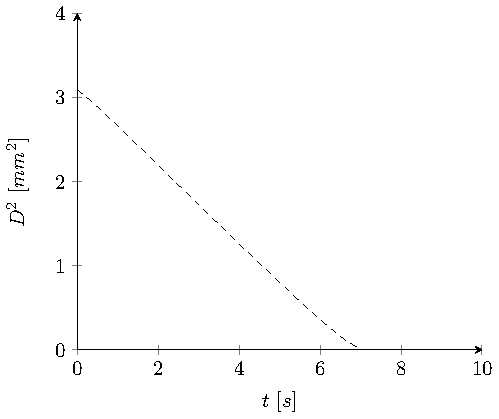
\includegraphics[width=0.8\textwidth]{./Diagrams/OpenCL_Coupled_Heat_Mass_Transfer_Verification/Coupled_D2_Transfer_Hexane.pdf}
		\caption{}
		\label{coupled_d2_hexane}
	\end{subfigure}
\end{figure}
\begin{figure}\ContinuedFloat
	\begin{subfigure}{\textwidth}
		\centering
		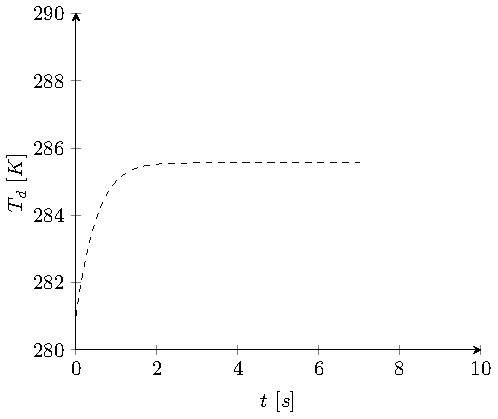
\includegraphics[width=0.8\textwidth]{./Diagrams/OpenCL_Coupled_Heat_Mass_Transfer_Verification/Coupled_Heat_Transfer_Hexane.pdf}
		\caption{}
		\label{coupled_heat_hexane}
	\end{subfigure}
	\caption{Droplet diameter squared (a) and droplet temperature (b) temporal evolution for a hexane droplet sized $D_0=1.76mm$ with $Re_d=110$, $T_{d_0}=281K$, $T_G=437K$ and $\Delta t=\tau_{d0}/64$.}
\end{figure}

\subsection{Decane Droplet}
\begin{figure}[H]
	\centering
	\begin{subfigure}{\textwidth}
		\centering
		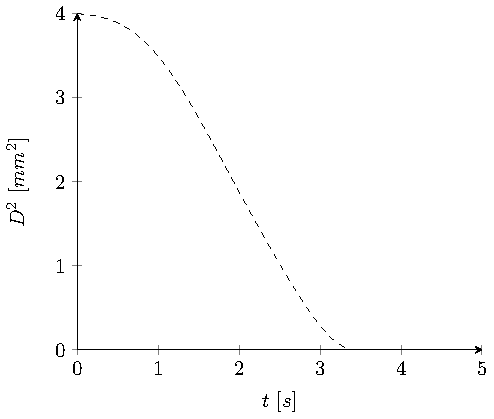
\includegraphics[width=0.8\textwidth]{./Diagrams/OpenCL_Coupled_Heat_Mass_Transfer_Verification/Coupled_D2_Transfer_Decane.pdf}
		\caption{}
		\label{coupled_d2_decane}
	\end{subfigure}
\end{figure}
\begin{figure}\ContinuedFloat
	\begin{subfigure}{\textwidth}
		\centering
		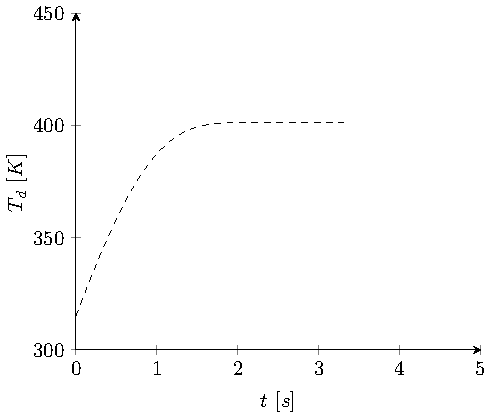
\includegraphics[width=0.8\textwidth]{./Diagrams/OpenCL_Coupled_Heat_Mass_Transfer_Verification/Coupled_Heat_Transfer_Decane.pdf}
		\caption{}
		\label{coupled_heat_decane}
	\end{subfigure}
	\caption{Droplet diameter squared (a) and droplet temperature (b) temporal evolution for a decane droplet sized $D_0=2.0mm$ with $Re_d=17$, $T_{d_0}=315K$, $T_G=1000K$ and $\Delta t=\tau_{d0}/64$.}
\end{figure}

\end{document}